\chapter{Hexagon Criterion}

We introduce the \emph{Hexagon Criterion}, first presented in \cite{bik2022classifying}, to determine whether subconfigurations of a chipsplitting outcome qualify as outcomes. This criterion applies to configurations supported within the yellow area below; we say the support is not contained inside the ``hexagon".

\begin{figure}[H]
    \centering
    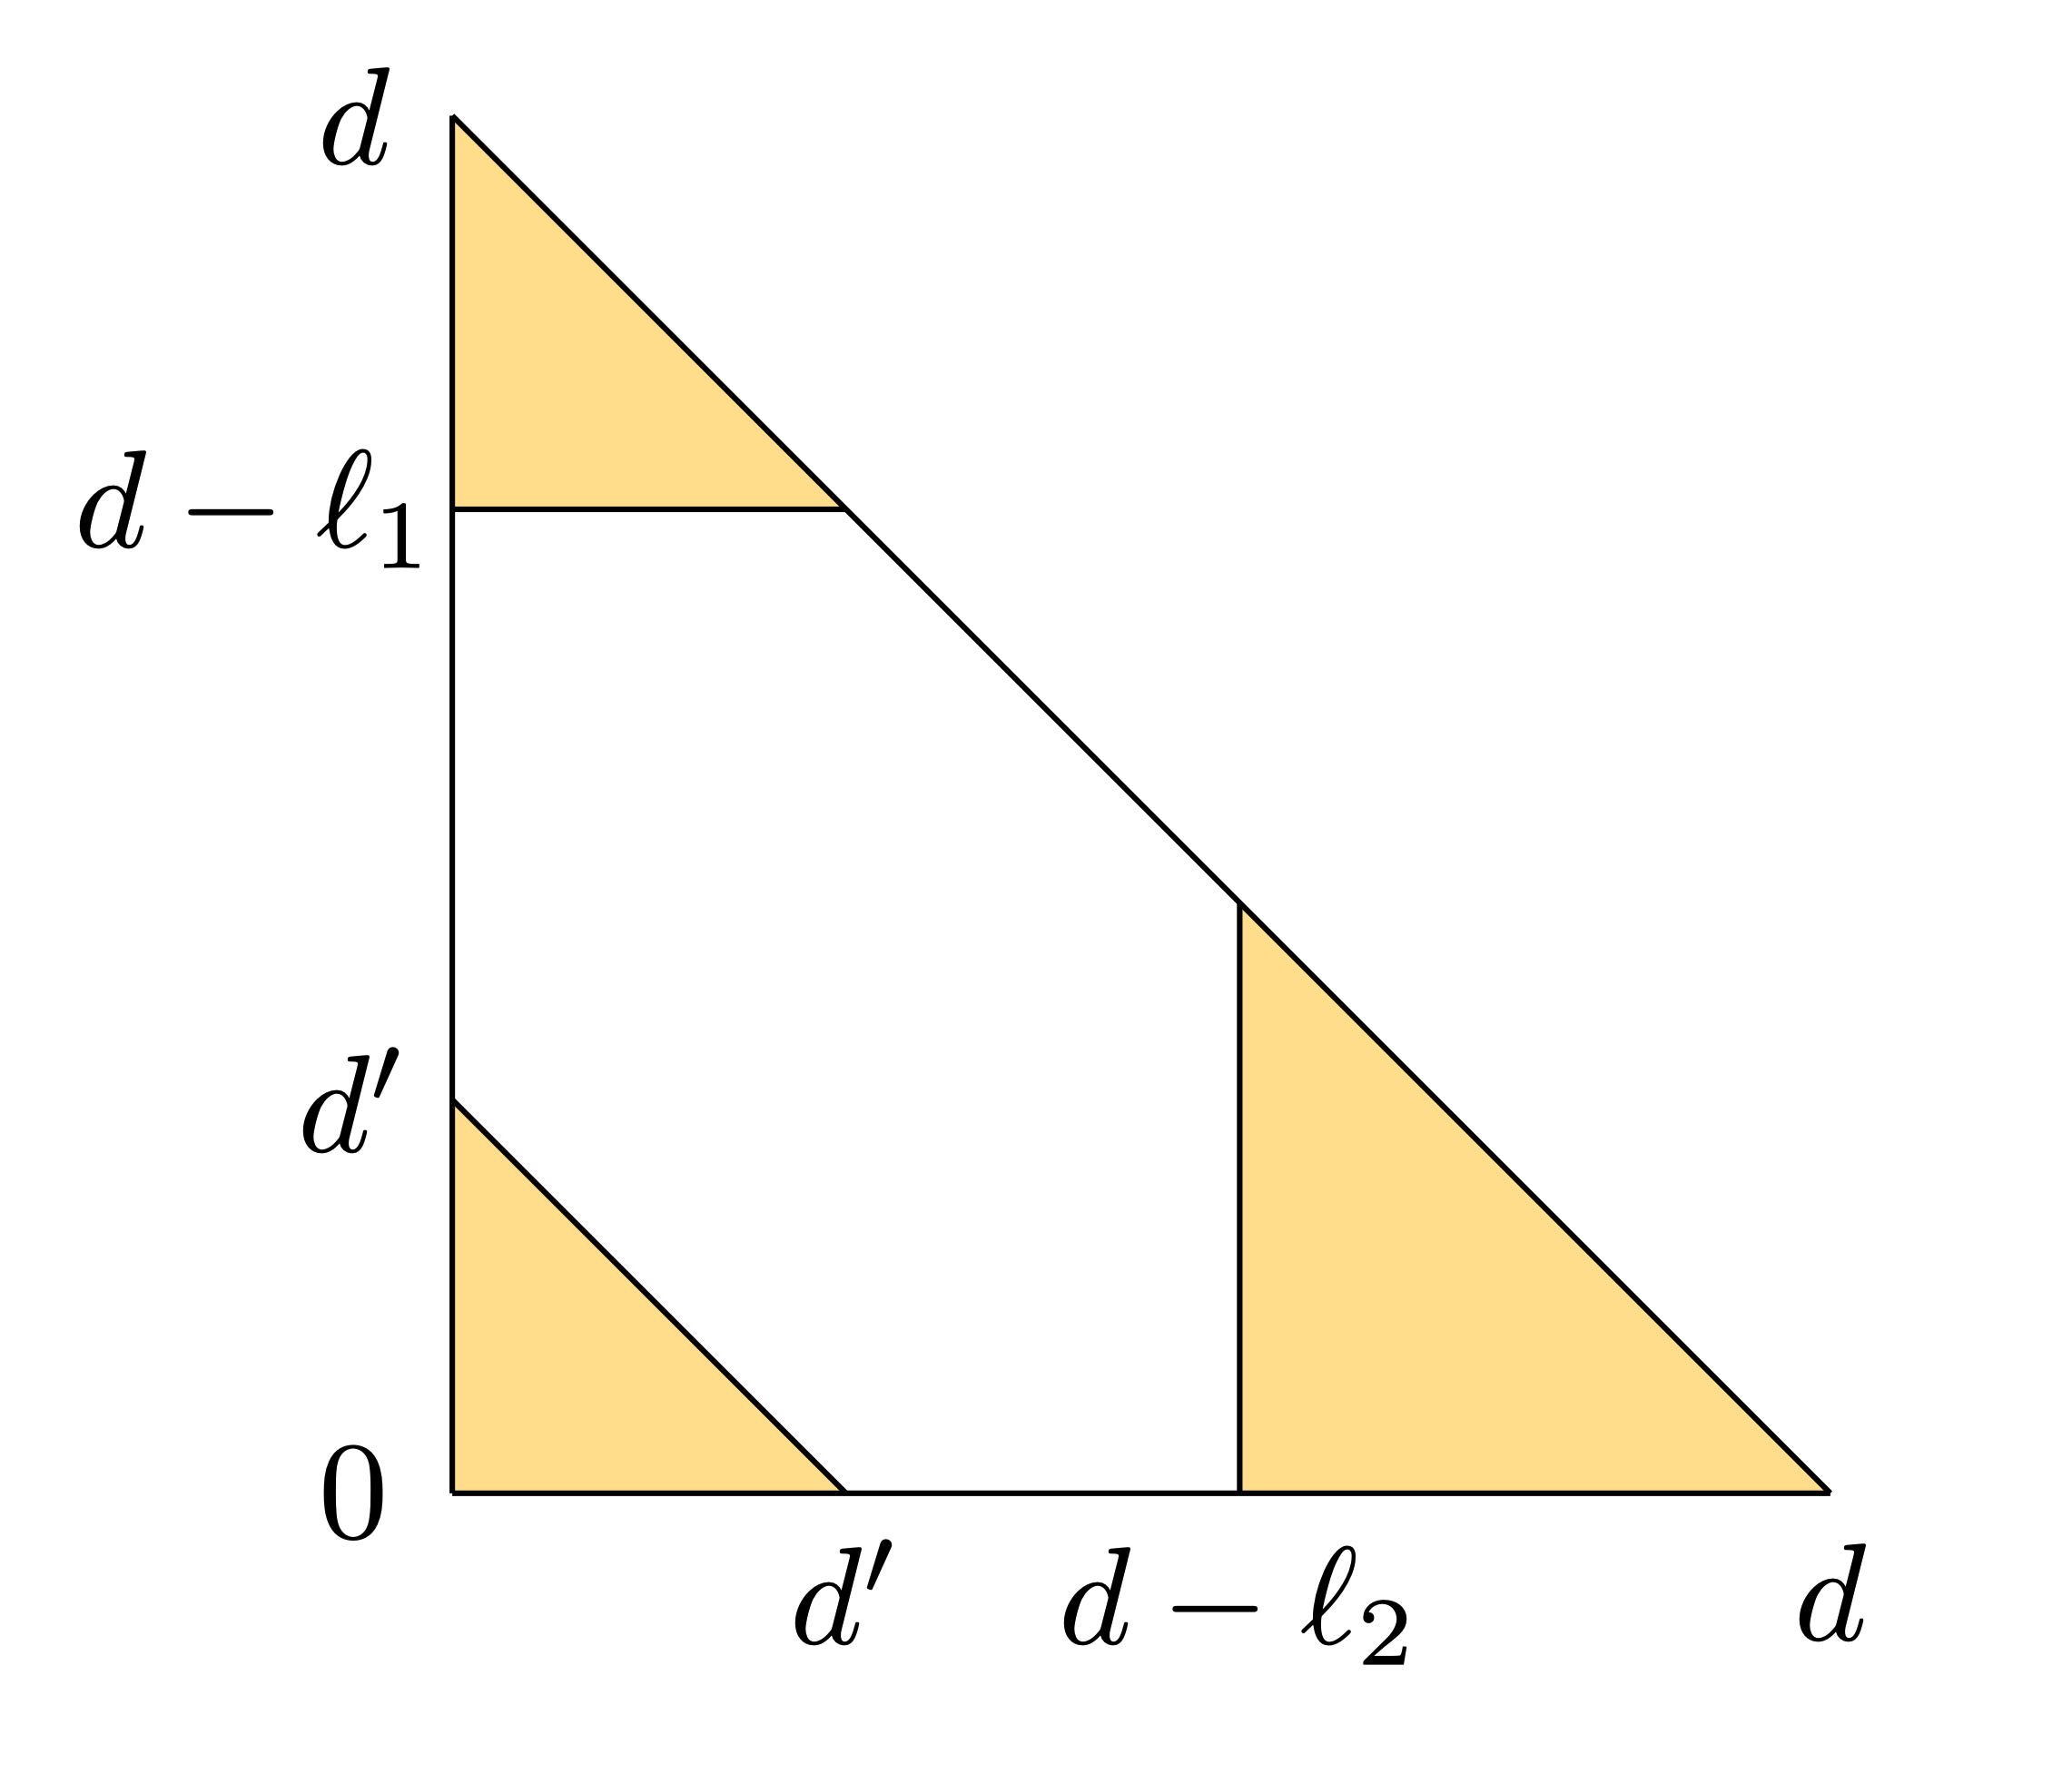
\includegraphics[width=0.4\textwidth]{assets/hexagon.png}
    \caption{A configuration's support lies outside the hexagon if it is contained in the yellow area spanned by parameters \( \ell_1, \ell_2 \), and \( d' \).}     \label{fig:hexagon}
\end{figure}

First, we need the following lemma to compute the determinant of matrix that we will encounter in the proof of the Hexagon Criterion.

\begin{lemma}\label{lemma:grinberghyperfactorial}
    Let \( a,b,c \in \mathbb{Z}_{\geq 0} \). Define the map \( H:  \mathbb{Z}_{\geq 0} \to  \mathbb{Z}_{\geq 0}, n \mapsto 0! 1! \cdots (n-1)! \); note that \( H(0) = 1 \). Then, the following holds:
    \begin{align*}
        \mathrm{det}\begin{bmatrix}
            \binom{a+b}{b-i+j}
        \end{bmatrix}_{i,j = 1}^c = \frac{H(a)H(b)H(c)H(a+b+c)}{H(b+c)H(c+a)H(a+b)}
    \end{align*} 
\end{lemma}

\begin{proof}
    See Theorem 8 of \cite{grinberghyperfactorial}.
\end{proof}


\begin{proposition}[Hexagon Criterion]\label{prop:hexagon-criterion231312}
    Let \( d, d', \ell_1, \ell_2 \in \mathbb{N} \) with \( d' \geq 1 \), \( \ell_1, \ell_2 \geq d' \), and \( d' + \ell_1 + \ell_2 \leq d \). Let \( \mathbf{w} = (w_{i,j})_{(i,j) \in V_d} \in \mathbb{Z}^{V_d} \) be a chip configuration. Define the subconfiguration \( \mathbf{w}' \coloneqq (w_{i,j})_{(i,j) \in V_{d'}} \in \mathbb{Z}^{V_{d'}}\). Assume the support of \( \mathbf{w} \) is not contained inside the ``hexagon" (see Figure \ref{fig:hexagon}), i.e. \( \mathrm{supp}(\mathbf{w}) \subset V_{d'}  \cup \left\{ (i,j) \in V_d \mid j > d - \ell_1 \right\} \cup \left\{ (i,j) \in V_d \mid i > d - \ell_2 \right\} \).
    Then, the following holds:
    \begin{enumerate}
        \item If \( \mathbf{w} \) is an outcome, then also its subconfiguration \( \mathbf{w}' \) is an outcome.
        \item If \( \mathbf{w} \) is a valid outcome, then \( \mathrm{deg}(\mathbf{w}) \leq d' \).
    \end{enumerate}
\end{proposition}

\begin{proof}
    We prove the first statement. Assume \( \mathbf{w} \) is an outcome. Let \( k = 0, \dots, d' \) and \( \mathrm{diag}(\ell_1 + k) = \sum_{(i,j) \in V_d} \mu_{i,j} x_{i,j} \). Consider the restricted linear form \( l_k = \sum_{(i,j) \in V_{d'}} \lambda_{i,j}x_{i,j} : \mathbb{Z}^{V_{d'}} \to \mathbb{Z} \) with \( \lambda_{i,j} \coloneqq \mu_{i,j} \) for \( (i,j) \in V_{d'} \). Then, \( l_0, \dots, l_{d'} \) are Pascal forms on \( \mathbb{Z}^{V_{d'}} \) with \( l_k(\mathbf{w}') = \mathrm{diag}(\ell_1 + k)(\mathbf{w}) = 0 \). By Proposition \ref{thm:pascal-outcome} it suffices to show that \( l_0, \dots, l_{d'} \) are linearly independent to show that \( \mathbf{w}' \) is an outcome.

    Let \( a = 0, \dots, d' \). Define
    \begin{align*}
        e_{{i,j}}^{(a)} &\coloneqq \begin{cases}
            1 & \text{ if } i = a \text{ and } j = d' - a, \\
            0 & \text{ otherwise}.
        \end{cases}\\
        A &\coloneqq \begin{bmatrix}
            l_k(\mathbf{e}^{(a)})
        \end{bmatrix}^{d'}_{k,a = 0} = \begin{bmatrix}
            \binom{d-d'}{\ell_1 + k - a}
        \end{bmatrix}^{d'}_{k,a = 0} = \begin{bmatrix}
            \binom{(d-d' - \ell_1) + \ell_1}{\ell_1 + k - a}
        \end{bmatrix}^{d'}_{k,a = 0}.
    \end{align*}
    We want to show that the matrix \( A \) is invertible because this implies that the linear forms \( l_0, \dots, l_{d'} \) are linearly independent. We observe that 
    \begin{enumerate}
        \item all entries of \( A \) are nonzero because \( 0 \leq \ell_1 + k - a \leq d - d' \), and 
        \item \( d - d' - \ell_1 \geq \ell_2 \geq 0 \).
    \end{enumerate}
    This allows us to use Lemma \ref{lemma:grinberghyperfactorial} with \( a \coloneqq d - d' - \ell_1, b \coloneqq \ell_1\), and \( c \coloneqq d' + 1 \).
    We obtain a nonzero determinant \( \mathrm{det}(A) = \frac{H(d - d' - \ell_1)H(\ell_1)H(d' + 1)H(d+1)}{H(\ell_1 + d' + 1)H(1 + d - \ell_1)H(d - d')} \neq 0 \).
    Hence, \( l_0, \dots, l_{d'} \) are linearly independent.

    For the second statement, let \( \mathbf{w} \) be a valid outcome. By the previous statement, the subconfiguration \( \mathbf{w}' \) is an outcome, as well. We extend \( \mathbf{w}' \) to some configuration \( \mathbf{v} \in \mathbb{Z}^{V_d} \) by \( v_{i,j} \coloneqq \begin{cases}
        w_{i,j}' & \text{ if } (i,j) \in V_{d'}, \\
        0 & \text{ otherwise}
    \end{cases} \).
    Clearly, \( \mathbf{v} \) is a \emph{valid} outcome of degree at most \( d' \). Then, \( \mathbf{v} - \mathbf{w} \) is an outcome with empty negative support. By Proposition \ref{prop:outcome-zero}, \(  \mathbf{v} - \mathbf{w} \) is zero. Hence, \( \mathbf{w} \) has degree at most \( d' \).
\end{proof}

